\documentclass[conference]{IEEEtran}
\IEEEoverridecommandlockouts
\usepackage[brazil]{babel}
\usepackage[utf8] {inputenc}
\usepackage{cite}
\usepackage{amsmath,amssymb,amsfonts}
\usepackage{algorithmic}
\usepackage{graphicx}
\usepackage{textcomp}
\usepackage{xcolor}
\def\BibTeX{{\rm B\kern-.05em{\sc i\kern-.025em b}\kern-.08em
T\kern-.1667em\lower.7ex\hbox{E}\kern-.125emX}}
\begin{document}

\title{Desenvolvimento de aplicação web para experimentar mobílias utilizando realidade aumentada\\
}

\author{
  \IEEEauthorblockN{Daniel Amorim Vilela de Salis}
  \IEEEauthorblockA{123.145\\
    \textit{Universidade Federal de São Paulo}\\
    \ São José dos Campos, São Paulo\\
    \ daniel.salis@unifesp.br} \\

}

\maketitle

\begin{abstract}
  Este artigo apresenta o desenvolvimento de uma aplicação web que utiliza Realidade Aumentada (AR)
  para proporcionar experiências imersivas aos usuários na visualização e interação com mobílias.
  A integração da AR com tecnologias como WebXR, Three.js, React e Next.js
  permitiu criar uma plataforma de e-commerce. Apesar das limitações identificadas,
  como a dependência de condições de iluminação e variações de desempenho,
  a aplicação demonstrou o potencial da Realidade Aumentada para transformar a experiência web tanto dos usuários quanto dos desenvolvedores.
\end{abstract}

\begin{IEEEkeywords}
  Realidade Aumentada,
  Aplicativos Web,
  Mobílias,
  E-commerce,
  WebXR,
  Three.js,
  React,
  Next.js,
  Experiências Imersivas,
  Interação do Usuário
\end{IEEEkeywords}

\section{Introdução}
A Extended Reality (XR) pode ser definida por um "termo guarda-chuva", que
engloba a Realidade Aumentada (AR), Realidade Virtual (VR) e Realidade Mista
(MR)[1], está transformando diversas áreas, como: entretenimento (atrações
temáticas, jogos e filmes), educação (visualização de conceitos complexos em
3D, realização de simulações práticas) e saúde (treinamentos médicos,
planejamento cirúrgico). A Realidade Aumentada, como componente da XR, se
demonstra útil por sua capacidade na sobreposição de informações digitais
fazendo com que um usuário por meio de um dispositivo interaja de maneira
única, mas ao mesmo tempo que ele não perca o senso de presença no mundo
real[2]. Essa interseção de AR com outras tecnologias expande as possibilidades
de aplicação, tornando-as ferramentas valiosas para inovação em múltiplos
setores.

\par
Neste artigo o enfoque será dado à como o e-commerce pode se aproveitar de uma
maior interatividade do usuário. Uma plataforma de vendas que adiciona AR a fim
de vender seus produtos propõe experiencias imersivas, ou seja, ao invés da
visualização estática é possível ver de maneira mais realista e detalhada como
objetos poderão ser dispostos. Utilizando técnicas de engenharia de software
(principalmente voltados para a web) com conceitos de realidade virtual foi
desenvolvida a plataforma ArMarketplace, visando a criação de um protótipo que
demostre o fluxo de compra de mobílias (seleção de produto, adição ao carrinho,
e finalização de compra) somado com a visualização das mesmas em 3D no ambiente
desejado.

\section{Metodologia}
Para Sommerville[3], um modelo de processo de software pode ser descrito comum
uma representação simplificada desse mesmo processo e ao utilizar o "Modelo em
Cascata" foram consideradas as atividades fundamentais de Definição dos
requisitos, Projeto de sistema e software, Implementação e teste, Integração e
testes de sistema, Operação e manutenção como fases distintas. Formando dessa
maneira, a sequencia dos passos a serem seguidos. Por se tratar de um projeto
de curta duração para a disciplina de Realidade Virtual e Aumentada, e com
apenas um desenvolvedor, esta foi a abordagem escolhida.

%----------------------------------------------------------------------------
\begin{figure}[h]
  \caption{O modelo em cascata [3]}

  \centering % para centralizarmos a figura
  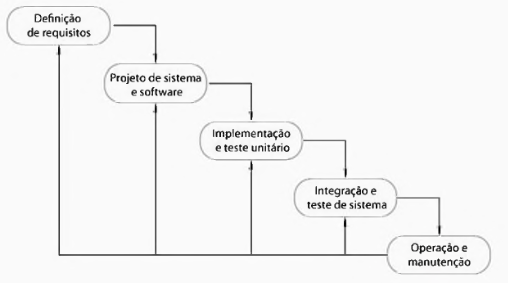
\includegraphics[width=8cm]{assets/modelo_cascata.png}
\end{figure}
%----------------------------------------------------------------------------

\subsection{Definição de requisitos}\label{AA}
São reconhecidos como serviços, restrições e metas de um sistema ao consultar
usuários. Neste trabalho como não houveram usuários formalmente consultados,
apenas outros marketplaces foram analisados para que o fluxo de navegação e
compra fosse similar (ex: Mercado Livre, Amazon, QueroBolsa). A figura [2]
mostra o diagrama de atividades que um usuário poderá seguir ao entrar na
plataforma. Buscando criar um design de referência da aplicação, um protótipo
foi desenvolvido utilizando a plataforma whimsical [8]. Protótipos visuais
(figura [3]) ajudam a identificar problemas de layout e usabilidade
precocemente, economizando tempo e recursos durante o desenvolvimento.

%----------------------------------------------------------------------------
\begin{figure}[h]
  \caption{Diagrama UML com os requisitos principais}

  \centering % para centralizarmos a figura
  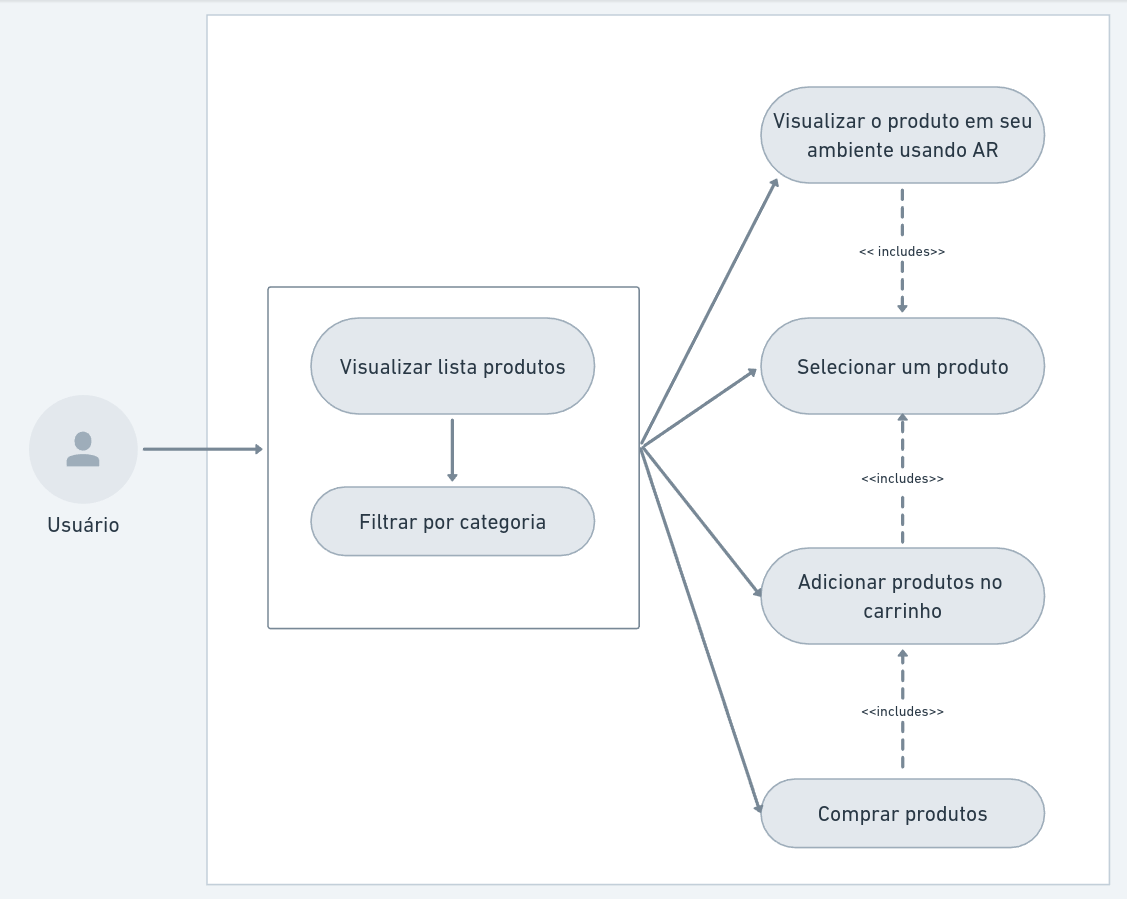
\includegraphics[width=8cm]{assets/user_uml_diagram.png}
\end{figure}
%----------------------------------------------------------------------------

%----------------------------------------------------------------------------
\begin{figure}[h]
  \caption{Design parcial da aplicação utilizando Whimsical}

  \centering % para centralizarmos a figura
  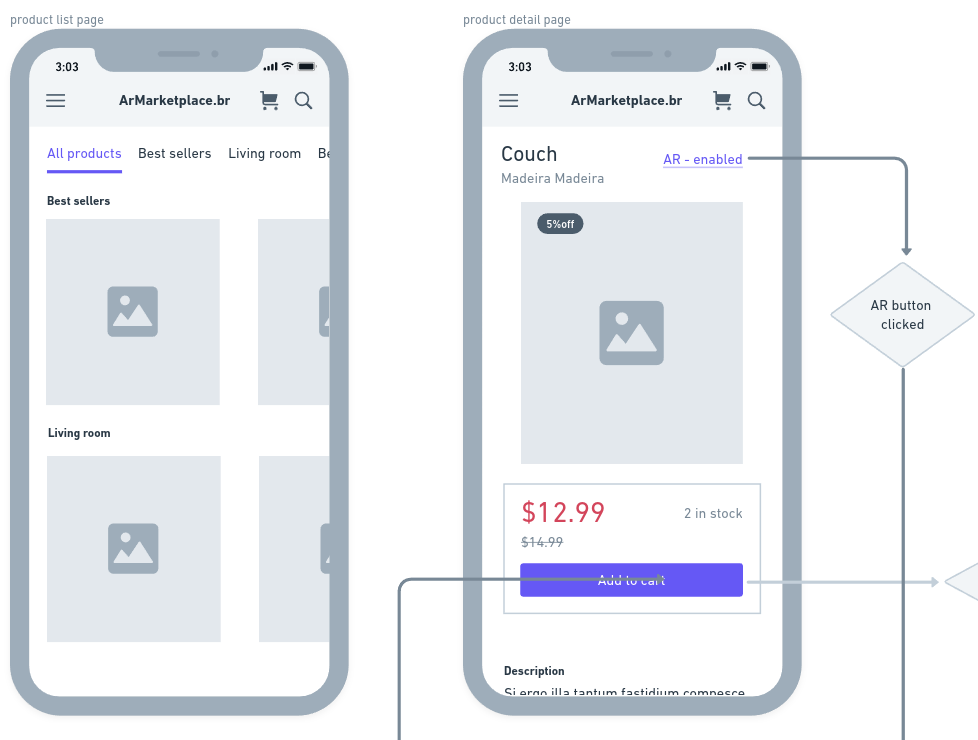
\includegraphics[width=8cm]{assets/design.png}
\end{figure}
%----------------------------------------------------------------------------

\subsection{Projeto de sistema e software}
O processo de projeto de sistemas busca distribuir os requisitos tanto para o
software, definindo uma arquitetura geral do sistema. Incluí também inclui a
identificação e descrição das abstrações fundamentais do sistema de software e
seus relacionamentos.
\par
Abaixo se encontram as linguagens e frameworks utilizados na construção do
software:
\begin{itemize}
  \item WebXR: Uma API que permite o desenvolvimento de experiências de realidade
        aumentada (AR) e realidade virtual (VR) diretamente nos navegadores da web [4].
  \item Three.js: Uma biblioteca JavaScript utilizada para criar e renderizar gráficos
        3D no navegador. Facilita a criação de cenas 3D complexas sem a necessidade de
        aprofundamentos em WebGL(a API de baixo nível para gráficos 3D na web)[5].
  \item React e Next.js: React é uma biblioteca JavaScript criada pelo Facebook para a
        construção de interfaces de usuário baseadas em componentes. Ela permite a
        criação de aplicações web utilizando uma abordagem declarativa para definir a
        interface de usuário[6]. Next.js é um framework de desenvolvimento web que
        utiliza React para a construção de aplicações ele visa facilitar a criação de
        aplicações React com funcionalidades como renderização do lado do servidor
        (SSR), geração estática de páginas (SSG) e roteamento simplificado[7].
  \item ShadCN é uma biblioteca de componentes UI projetada para fornecer elementos de
        interface de usuário funcionais para aplicações web[9].
\end{itemize}

\subsection{Implementação e teste unitário}
Durante esse estágio, o projeto do software é desenvolvido como um conjunto de
programas ou unidades de programa. Para isso foi utilizado como IDE (Integrated
Development Environment) o Visual Studio Code. Os testes unitários não foram
implementados devido ao pequeno escopo do projeto.
\par Ao utilizar Next.js os dois diretórios mais importantes da aplicação são: "app"
e o diretório "components". O diretório "app" é responsável por conter
subdiretórios que representam diferentes seções, funcionalidades ou layouts
principais da aplicação. "Components" é onde se organizam códigos reutilizáveis
de interface do usuário (UI). Todos os elementos de UI importados da biblioteca
ShadCN foram armazenados neste diretório.

\subsection{Integração e teste de sistema}
As unidades do programa ou programas são solidificadas e testadas como um
sistema completo para assegurar que os requisitos do software tenham sido
atendidos. Após o teste, o sistema de software pode ser entregue ao "cliente".
As figuras [4][5][6] mostram os resultado do desenvolvimento das páginas:
inicial, de descrição de produto e teste do produto
%----------------------------------------------------------------------------
\begin{figure}[h]
  \caption{Página inicial}

  \centering % para centralizarmos a figura
  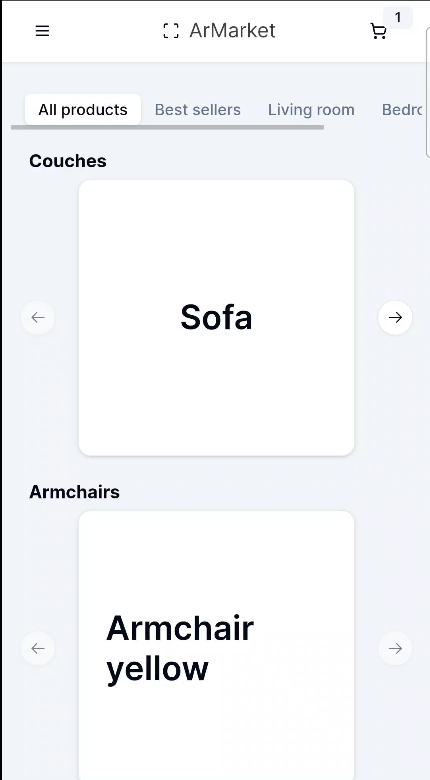
\includegraphics[width=4cm]{assets/home_page.png}
\end{figure}
%----------------------------------------------------------------------------
%----------------------------------------------------------------------------
\begin{figure}[h]
  \caption{Página de produto}

  \centering % para centralizarmos a figura
  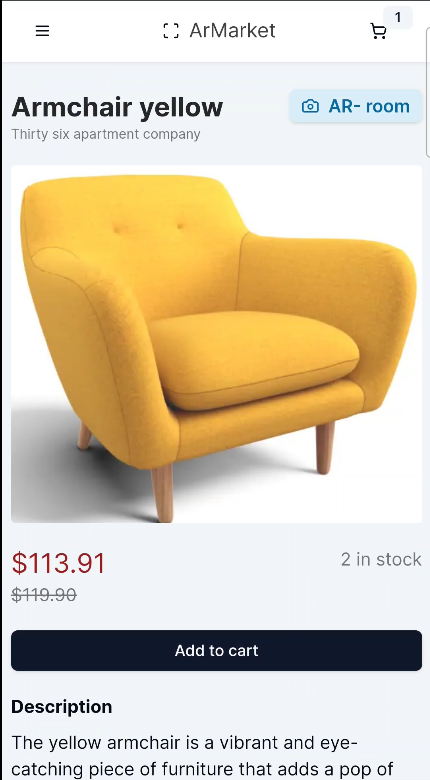
\includegraphics[width=4cm]{assets/product_page.png}
\end{figure}
%----------------------------------------------------------------------------
%----------------------------------------------------------------------------
\begin{figure}[h]
  \caption{Página de realidade aumentada}

  \centering % para centralizarmos a figura
  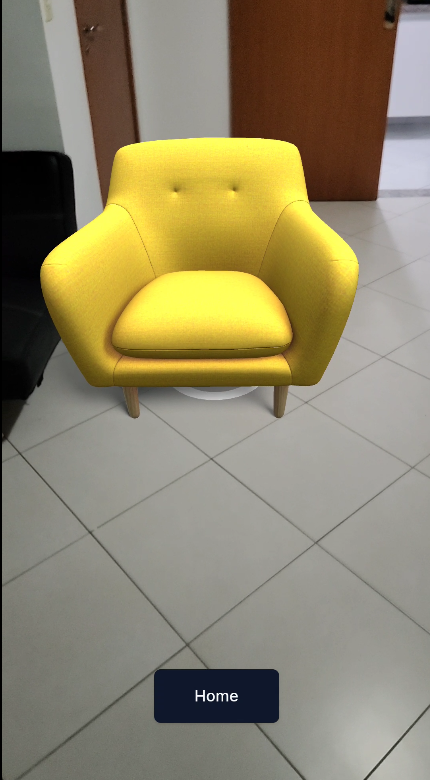
\includegraphics[width=4cm]{assets/test_page.png}
\end{figure}
%----------------------------------------------------------------------------

\subsection{Operação e manutenção}
Nessa etapa o sistema está pronto para uso, a manutenção envolve a correção de
erros que não foram descobertos em estágios iniciais do ciclo de vida, com
melhora da implementação das unidades do sistema e ampliação de seus serviços
em resposta às descobertas de novos requisitos. Como o caráter deste artigo é
apenas demonstrativo a aplicação não foi enviada ao chamado "ambiente de
produção"

\section{Resultados}
Com a conclusão da implementação a aplicação pode permitir aos usuários seguir
fluxos de seleção de produtos, inseri-los em seu ambiente real e concluir
compras. A seguir, os resultados são melhor detalhados:

\subsection{Seleção de Produtos}\label{AA}
Os usuários podem navegar por uma lista de produtos disponíveis no marketplace,
podendo ser filtrados por categorias pré-definidas.

\subsection{Inserção no Ambiente Real}\label{AA}
API WebXR em conjunto com Three.js garantiu a fluidez e rapidez dessa
funcionalidade. Ao clicar em um produto, o usuário é redirecionado para a
página de detalhamento do produto e sendo inserir modelos 3D dos produtos
selecionados nesta página em seu ambiente real, posicionando-os onde achar
melhor.

\subsection{Conclusão de compra}\label{AA}
Também foram concluídas as páginas de "carrinho de compras" e "finalização de
compra", sendo possível revisar o pedido (preços e taxa de entrega) e concluir
a compra das mobílias selecionadas previamente, figura[7].

%----------------------------------------------------------------------------
\begin{figure}[h]
  \caption{Página de revisão do pedido}

  \centering % para centralizarmos a figura
  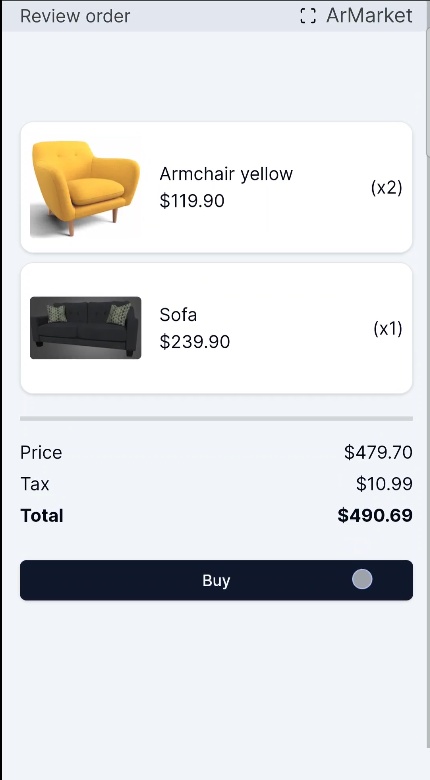
\includegraphics[width=4cm]{assets/review_page.png}
\end{figure}
%----------------------------------------------------------------------------

\section{Conclusão}
O desenvolvimento de uma pequena plataforma de marketplace utilizando Nuxt, a
api WebXR e threejs demonstrou ser uma ideia em potencial que pode ser
implementada em lojas que visam surpreender os clientes com uma nova abordagem
de venda. A aplicação permite aos usuários selecionar produtos, visualizá-los
em seu ambiente real utilizando tecnologia AR, e concluir compras diretamente
pelo navegador, sem a necessidade de instalar um aplicativo nativo.

\par Apesar do resultado obtido, algumas limitações foram identificadas, como a
dependência de boas condições de iluminação para a precisão da colocação dos
objetos 3D e variações de desempenho entre diferentes dispositivos. Além
disso,no momento os modelos renderizados são carregados dentro do "front-end"
da aplicação, devido ao peso de cada arquivo para trabalhos futuros será
importante a criação de um mecanismo que proporcione o carregamento através do
servidor (evitando que a página utilize muitos dados do usuário). Estas áreas
representam oportunidades para futuras otimizações, como aprimoramentos nos
algoritmos de detecção de luz ambiente e otimizações de performance para
garantir uma experiência uniforme em uma gama mais ampla de dispositivos.

\par A integração de React com WebXR e Three.js proporcionou uma arquitetura modular
e escalável, facilitando e provando que aplicações web tem potencial para
transformar tanto a experiencia do usuário quando do desenvolvedor.

%----------------------------------------------------------------------------
\begin{thebibliography}{00}
  \bibitem{b}L. Tremosa. “Beyond AR vs. VR: What is the Difference between AR vs. MR vs. VR vs. XR?” Interaction Design Foundation - IxDF. https://www.interaction-design.org/literature/article/beyond-ar-vs-vr-what-is-the-difference-between-ar-vs-mr-vs-vr-vs-xr (accessed May. 30, 2024).

  \bibitem{b}J. Y. Ma and J. S. Choi, "The Virtuality and Reality of Augmented Reality," Journal of Multimedia, vol. 2, no. 1, pp. 32-37, 2007.

  \bibitem{sommerville2011engenharia}I. Sommerville, \emph{Engenharia de Software}. Pearson Prentice Hall, 2011. Available: https://books.google.com.br/books?id=H4u5ygAACAAJ

  \bibitem{immersiveweb}
  The Immersive Web Community Group, "Immersive Web," [Online]. Available: https://immersiveweb.dev/. [Accessed: 30-May-2024].

  \bibitem{threejs}
  Mr. Doob, "Three.js – JavaScript 3D library," [Online]. Available: https://threejs.org/. [Accessed: 30-May-2024].

  \bibitem{react}
  Facebook Inc., "React – A JavaScript library for building user interfaces," [Online]. Available: https://react.dev/. [Accessed: 30-May-2024].

  \bibitem{nextjs}
  Vercel Inc., "Next.js – The React Framework for Production," [Online]. Available: https://nextjs.org/. [Accessed: 30-May-2024].

  \bibitem{whimsical}
  Whimsical, "Whimsical - The Visual Workspace," Available: https://whimsical.com/. [Accessed: May 30, 2024].

  \bibitem{shadcn}
  ShadCN. (2024). ShadCN UI - Beautifully designed components for your web applications. [Online]. Available: https://ui.shadcn.com/

  \bibitem{qu2020}
  C. Qu and L. Aflatoony, "An Augmented Reality Design Tool to Guide Furniture Arrangements at Home," in \textit{Proceedings of the IEEE Conference on Virtual Reality and 3D User Interfaces}, 2020.

  \bibitem{ARFurniture}
  W. Viyanon, T. Songsuittipong, P. Piyapaisarn, S. Sudchid,
  ``AR Furniture: Integrating Augmented Reality Technology to Enhance Interior Design using Marker and Markerless tracking,''
  \emph{Department of Computer Science, Faculty of Science, Srinakharinwirot University, Bangkok, Thailand},
  waraporn@g.swu.ac.th.

  \bibitem{khandecal}
  S.~Khan, A.~Mahadik, A.~Pal, and S.~Jacob, ``‘Decal App’-Augmented Reality based Flutter Application,'' \emph{Journal of Augmented Reality}, vol.~1, no.~1, pp.~1--10, 2024.

  \bibitem{phan2010interior}
  V. T. Phan and S. Y. Choo, "Interior design in augmented reality environment," *International Journal of Computer Applications*, vol. 5, no. 5, pp. 16-21, 2010.

  \bibitem{poudel2018interior}
  A. Poudel and O. Al-Azzam, "Interior design with augmented reality," in \textit{Midwest Instr. Comput. Symp.}, 2018.

  \bibitem{ma2007virtuality}
  J. Y. Ma and J. S. Choi, "The Virtuality and Reality of Augmented Reality," \textit{J. Multim.}, vol. 2, no. 1, pp. 32-37, 2007.

  \bibitem{rzeszewski2021usability}
  M. Rzeszewski and M. Orylski, "Usability of WebXR visualizations in urban planning," \textit{ISPRS International Journal of Geo-Information}, vol. 10, no. 11, p. 721, 2021.
\end{thebibliography}

\end{document}
